 
\chapter{从实验角度理解工具变量法}
 \label{chapter::iv-experiment}



{\it 工具变量方法}是计量经济学中的有力工具，能够在处理与结果之间存在混杂时识别因果效应。它依赖一个满足特定条件的额外变量，即{\it 工具变量}（IV）。初学时，这些条件可能不易理解，使工具变量方法显得有些神奇。本章从鼓励设计出发，给出一种并不神秘的解释。这也再次呼应了\citet{dorn1953philosophy}的建议：规划观察性研究时，应始终问自己下面的问题。\footnote{第\ref{chapter::observational-studies}章已经引用过这段话。}
\begin{quote}
如果能够通过受控实验来完成研究，那么实验应当如何开展呢？
\end{quote} 
工具变量方法在实验中的对应问题是{\it 不依从}，它出现在{\it 鼓励设计}中\citep{zelen1979new, powers1984effects, holland1986statistics}。 



\section{激励设计与不遵从行为}

考虑一项单位编号为$i = 1,\ldots, n$的实验。令$Z_i$表示分配的处理，$1$表示处理、$0$表示对照；令$D_i$表示实际接受的处理，$1$表示处理、$0$表示对照。若某个单位$i$满足$Z_i \neq D_i$，就出现了不依从问题。不依从非常常见，尤其是在以人为实验单位的鼓励设计中。此时实验者不能强迫单位接受处理，只能鼓励其接受。令$Y_i$表示所关心的结果。 

考虑对$Z$进行完全随机化，暂不考虑协变量$X$。相对于分配水平$1$与$0$，实际接受处理的潜在取值为$\{  D_i(1), D_i(0) \}$，结果的潜在取值为$\{ Y_i(1), Y_i(0)  \}$。它们的观测值分别为$D_i = Z_i D_i(1) + (1-Z_i) D_i(0)$和$Y_i = Z_i Y_i(1) + (1-Z_i) Y_i(0)$。为简化记号，假设$\{  Z_i, D_i(1), D_i(0) ,Y_i(1), Y_i(0)  \}_{i=1}^n \iidsim \{  Z, D(1), D(0) ,Y(1), Y(0)  \}$，并在不致混淆时省略下标$i$。 


先从完全随机实验开始。 
\begin{assumption}[随机化]
\label{assume::random}
$Z\ind \{D(1), D(0) ,Y(1), Y(0)   \}$. 
\end{assumption}

随机化使$D$和$Y$上的平均因果效应可识别：
$$
\tau_D = E\{  D(1) - D(0) \} = E(D\mid Z=1) - E(D \mid Z=0)
$$
以及
$$
\tau_Y = E\{  Y(1) - Y(0) \} = E(Y\mid Z=1) - E(Y\mid Z=0).  
$$
可分别用简单均值差估计量$\hat{\tau}_D$与$\hat{\tau}_Y$估计$\tau_D$与$\tau_Y$。 


报告估计值$\hat{\tau}_Y$及其标准误，称为意向治疗（ITT）分析。它估计处理分配对结果的效应，假设\ref{assume::random}中的完全随机实验设计保证了这一分析的有效性。但它未必回答真正的科学问题，即实际接受的处理对结果有何因果效应。 




\section{潜在依从状态与效应}

\subsection{非参数识别}


遵循\citet{imbens1994identification}和\citet{angrist1996identification}，按联合潜在取值$U_i = \{  D_i(1), D_i(0) \}$对总体分层。由于$D$为二元变量，共有四种组合：
\begin{eqnarray*}
U_i=\left \{ \begin{array} {ll}
\at  , & \text{if} \hspace{2mm} D_i(1)=1 \hspace{2mm} \text{and} \hspace{2mm} D_i(0)=1; \\
\cp  , & \text{if} \hspace{2mm} D_i(1)=1 \hspace{2mm} \text{and} \hspace{2mm} D_i(0)=0; \\
\df  ,& \text{if} \hspace{2mm} D_i(1)=0 \hspace{2mm} \text{and} \hspace{2mm} D_i(0)=1; \\
\nt  , & \text{if} \hspace{2mm} D_i(1)=0 \hspace{2mm} \text{and} \hspace{2mm} D_i(0)=0,
\end{array}
\right.  
\end{eqnarray*}
其中“$\at$”表示始终接受者，“$\cp$”表示依从者，“$\df$”表示反向依从者，“$\nt$”表示从不接受者。由于不能同时观测$D_i(1)$与$D_i(0)$，$U_i$是描述单位$i$依从行为的潜变量。 


根据$U$，用全概率公式可将$Y$上的平均因果效应分解为四项：
\begin{eqnarray} 
\tau_Y &=& E\{ Y(1) - Y(0) \mid U=\at  \} \pr(U = \at )  \nonumber  \\
&&+ E\{ Y(1) - Y(0) \mid U=\cp   \} \pr(U = \cp ) \nonumber  \\
&&+ E\{ Y(1) - Y(0) \mid U=\df  \} \pr(U = \df ) \nonumber  \\
&&+ E\{ Y(1) - Y(0) \mid U=\nt  \} \pr(U = \nt ) . \label{eq::decompose-ate-y-cace}
\end{eqnarray}
因此，$\tau_Y $是四个潜在亚组效应的加权平均。下面详细考察这些潜在亚组。 



下面的假设\ref{assume::Mono}将\eqref{eq::decompose-ate-y-cace}中的第三项限制为零。 
\begin{assumption}[单调性]
\label{assume::Mono}
对所有$i$，$\pr(U_i = \df) = 0$，或等价地，$D_i(1)\geq D_i(0)$，即不存在反向依从者。 
\end{assumption}

在{\it 单侧不依从}情形下，假设\ref{assume::Mono}自动成立：分配到对照组的单位无法获得处理，即所有单位都满足$D_i(0) = 0$。在随机化下，假设\ref{assume::Mono}蕴含可检验的限制
\begin{equation}
\label{eq::test-mono}
\pr(D=1\mid Z=1) \geq \pr(D=1\mid Z=0).
\end{equation}
但假设\ref{assume::Mono}远强于不等式\eqref{eq::test-mono}：前者在个体层面对$D_i(1)$与$D_i(0)$施加限制，后者只限制其平均水平。不过，只要可检验的限制\eqref{eq::test-mono}成立，就不能用观测数据反驳假设\ref{assume::Mono}。 


下面的假设\ref{assume::ER}要求处理分配只能通过实际接受的处理影响结果，从而将\eqref{eq::decompose-ate-y-cace}中的第一项和最后一项限制为零。 
\begin{assumption}[排除限制]
\label{assume::ER}
对于满足$U_i=\at$的始终接受者和满足$U_i = \nt$的从不接受者，均有$Y_i(1) = Y_i(0)$。 
\end{assumption}


假设\ref{assume::ER}的等价表述是：对所有$i$，$D_i(1) =  D_i(0)$必然蕴含$Y_i(1) =  Y_i(0)$。它要求处理分配只有在改变实际接受的处理时，才可能改变结果。在双盲随机对照试验中，这从生物学上通常是合理的，因为结果只依赖实际接受的处理。\footnote{一般应尽量实施盲法，以避免安慰剂效应、患者预期等带来的偏差。双盲试验中医生和患者都不知道处理分配；单盲试验中患者不知道，而医生知道。有时双盲甚至单盲都无法实施，这类试验称为开放试验。}也就是说，若处理分配不改变实际接受的处理，就也不改变结果。若处理分配存在不经由实际接受处理而影响结果的{\it 直接效应}，该假设就可能被违反。\footnote{这里非正式地使用“直接效应”一词，详见后文第\ref{chapter::mediation}和\ref{chapter::cde}章。}例如，非双盲随机对照试验中，处理分配可能通过未知途径影响结果。 





在假设\ref{assume::Mono}与\ref{assume::ER}下，分解式\eqref{eq::decompose-ate-y-cace}只剩第二项：
\begin{eqnarray}
\label{eq::aceY}
\tau_Y  = E\{ Y(1) - Y(0) \mid U=\cp   \} \pr(U = \cp ).
\end{eqnarray}
类似地，$D$上的平均因果效应可分解为四项：
\begin{eqnarray*}
\tau_D &=& E\{ D(1) - D(0) \mid U=\at  \} \pr(U = \at ) \\
&&+ E\{ D(1) - D(0) \mid U=\cp   \} \pr(U = \cp ) \\
&&+ E\{ D(1) - D(0) \mid U=\df  \} \pr(U = \df ) \\
&&+ E\{ D(1) - D(0) \mid U=\nt  \} \pr(U = \nt )  \\
&=& 0\times \pr(U = \at ) 
+ 1 \times \pr(U = \cp ) 
+ (-1)\times   \pr(U = \df )
+ 0 \times  \pr(U = \nt ) ,
\end{eqnarray*}
在假设\ref{assume::Mono}下简化为
\begin{eqnarray}
\label{eq::aceD}
\tau_D  = \pr(U = \cp ) .
\end{eqnarray}
由\eqref{eq::aceD}，依从者比例$\pi_\cp = \pr(U = \cp)$等于处理分配对$D$的平均因果效应，后者在完全随机实验中可识别。虽然不能根据观测数据确定哪些单位是依从者，但可由\eqref{eq::aceD}识别他们在总体中的比例。结合\eqref{eq::aceY}与\eqref{eq::aceD}，得到以下结论。


\begin{theorem}
\label{thm::CACE-identification}
在假设 \ref{assume::Mono} 与 \ref{assume::ER} 成立时，若 $\tau_D \neq 0$，则有 
$$
E\{ Y(1) - Y(0) \mid U=\cp   \} = \frac{ \tau_Y  }{ \tau_D}
$$ 
\end{theorem}


 

参考 \citet{imbens1994identification} 与 \citet{angrist1996identification} 的定义，我们定义

\begin{definition}[CACE 或 LATE]\label{def::CACE}
定义 
$$
\tau_\cp  =  E\{ Y(1) - Y(0) \mid U=\cp   \}  
$$
为“遵从者平均因果效应”或“局部平均处理效应”。该量亦可用下式表达：
\begin{eqnarray*}
\tau_\cp  &=&  E\{ Y(1) - Y(0) \mid D(1) = 1 , D(0) = 0  \} \\
&=&    E\{ Y(1) - Y(0) \mid D(1)  >  D(0)    \} . 
\end{eqnarray*}
\end{definition}

CACE 是满足$ D(1) = 1 , D(0) = 0$的依从者中$Z$对$Y$的平均因果效应；在单调性下，依从者也等价于满足$ D(1)  >  D(0)$的单位。由定义\ref{def::CACE}，定理\ref{thm::CACE-identification}可改写为
$$
\tau_\cp  = \frac{ \tau_Y  }{ \tau_D} ,
$$
即 CACE 或 LATE 等于$Y$上的平均因果效应与$D$上的平均因果效应之比。在假设\ref{assume::random}下，进一步得到如下 CACE 识别结果。


\begin{corollary}
\label{corollary::identification-CACE}
在假设 \ref{assume::random} 至 \ref{assume::ER} 均成立时，有
$$
\tau_\cp = \frac{ E(Y\mid Z=1) - E(Y\mid Z=0) }{ E(D\mid Z=1) - E(D \mid Z=0) } .
$$
\end{corollary}


因此，在完全随机实验、单调性与排除限制假设下，CACE 可通过结果均值差与处理均值差之比来非参数地估计。 



\subsection{估计方法}
\label{sec::estimation-IV}


根据推论\ref{corollary::identification-CACE}，可用简单比值
$$
\hat{\tau}_\cp  = \frac{  \hat{\tau}_Y }{  \hat{\tau}_D  } ,
$$
估计$\tau_\cp$，这称为 Wald 估计量\citep{wald1940fitting}或工具变量估计量。上述讨论中，$Z$是$D$的工具变量。   



可用下面的直观推导得到方差估计量（见例\ref{thm::delta-method}）：
$$
\hat{\tau}_\cp - \tau_\cp  = ( \hat{\tau}_Y  -  \tau_\cp\hat{\tau}_D)/\hat{\tau}_D 
\approx  ( \hat{\tau}_Y  -  \tau_\cp\hat{\tau}_D)/ \tau_D 
= \hat{\tau}_A / \tau_D ,
$$
其中$\hat{\tau}_A$是调整后结果$A_i = Y_i -  \tau_\cp D_i$的均值差。因此，$\hat{\tau}_\cp$的渐近方差近似等于$\hat{\tau}_A$的方差除以$\tau_D^2$。方差估计分以下几步进行： 
\begin{enumerate}
%[(\thesection.1)]
\item
计算调整后的结果变量 $\hat{A}_i =  Y_i -  \hat{\tau}_\cp D_i\ (i=1, \ldots, n)$；

\item
计算 Neyman 型方差估计值：
$$
\hat{V}_{\hat{A}} = \frac{\hat{S}_{\hat{A}}^2(1)}{n_1} + \frac{\hat{S}_{\hat{A}}^2(0)}{n_0},
$$
其中 $\hat{S}_{\hat{A}}^2(1)$ 与 $\hat{S}_{\hat{A}}^2(0)$ 分别为实验组与对照组下 $\hat{A}_i $ 的样本方差； 

\item
最终得到方差估计值 $ \hat{V}_{\hat{A}} /  \hat{\tau}_D ^2 .$ 
\end{enumerate}


上述方差估计量的论证见习题\ref{problem::var-iv-estimate}。也可用自助法近似$\hat{\tau}_\cp $的方差。下面的函数计算点估计$\hat{\tau}_\cp $，以及基于公式$\hat{V}_{\hat{A}} $和自助法的标准误。 

\begin{lstlisting}
## IV point estimator
IV_Wald = function(Z, D, Y)
{
       tau_D = mean(D[Z==1]) - mean(D[Z==0])
       tau_Y = mean(Y[Z==1]) - mean(Y[Z==0])
       CACE  = tau_Y/tau_D
       
       c(tau_D, tau_Y, CACE)
}

## IV se via the delta method
IV_Wald_delta = function(Z, D, Y)
{
       est         = IV_Wald(Z, D, Y)
       AdjustedY   = Y - D*est[3]
       VarAdj      = var(AdjustedY[Z==1])/sum(Z) + 
                          var(AdjustedY[Z==0])/sum(1 - Z)
       
       c(est[3], sqrt(VarAdj)/abs(est[1]))
}

##IV se via the bootstrap
IV_Wald_bootstrap = function(Z, D, Y, n.boot = 200)
{
       est      = IV_Wald(Z, D, Y)
       
       CACEboot  = replicate(n.boot, {
         id.boot = sample(1:length(Z), replace = TRUE)
         IV_Wald(Z[id.boot], D[id.boot], Y[id.boot])[3]
       })
       
       c(est[3], sd(CACEboot))
}
\end{lstlisting}


在零假设$\tau_\cp = 0$下，可用$\hat{V}_Y /  \hat{\tau}_D ^2$近似方差，其中$\hat{V}_Y$是$Y$均值差的 Neyman 型方差估计。若真实的$\tau_\cp$不为零，这个方差估计量就不一致，因此适用于检验而非一般估计。不过，它揭示了 ITT 估计量与 Wald 估计量的关系。ITT 估计量$\hat{\tau}_Y$的估计标准误为$\sqrt{ \hat{V}_Y}$。Wald 估计量$ \hat{\tau}_Y / \hat{\tau}_D$相当于将 ITT 估计量乘以$1/\hat{\tau}_D > 1$，其绝对值更大，但估计标准误也扩大相同倍数。根据方差估计$\hat{V}_Y $和$\hat{V}_Y /  \hat{\tau}_D ^2$，$\tau_Y$与$\tau_\cp$的置信区间分别为
$$
\hat{\tau}_Y \pm z_{1-\alpha/2} \sqrt{ \hat{V}_Y}
$$
和
$$
\hat{\tau}_Y  / \hat{\tau}_D \pm z_{1-\alpha/2} \sqrt{ \hat{V}_Y}  / \hat{\tau}_D
= 
\left( \hat{\tau}_Y \pm z_{1-\alpha/2} \sqrt{ \hat{V}_Y}  \right) / \hat{\tau}_D 
$$
其中$z_{1-\alpha/2}$是标准正态分布的$1-\alpha/2$分位数。这两个区间给出相同的定性结论：要么都包含零，要么都不包含零。从这个意义上说，尽管工具变量分析更复杂，它提供的定性信息与对$Y$作 ITT 分析相同。  




\section{协变量的作用}

\subsection{完全随机实验中的协变量调整}

现在考虑带有协变量的完全随机实验，假设
$$
Z\ind \{ D(1), D(0), Y(1), Y(0), X \}.
$$
利用协变量$X$，可分别对$D$和$Y$计算\citet{lin2013}提出的估计量$\hat{\tau}_{D,\textsc{L}}$与$\hat{\tau}_{Y,\textsc{L}}$，从而得到$\hat{\tau}_{\cp, \textsc{L}} = \hat{\tau}_{Y,\textsc{L}} / \hat{\tau}_{D,\textsc{L}}$。可用自助法近似$\hat{\tau}_{\cp, \textsc{L}} $的渐近方差。下面的函数计算点估计$\hat{\tau}_{\cp, \textsc{L}} $及其自助法标准误。 
 
\begin{lstlisting}
## covariate adjustment in IV analysis
IV_Lin = function(Z, D, Y, X)
{
  X     = scale(as.matrix(X))
  tau_D = lm(D ~ Z + X + Z*X)$coef[2]
  tau_Y = lm(Y ~ Z + X + Z*X)$coef[2]
  CACE  = tau_Y/tau_D
  
  c(tau_D, tau_Y, CACE)
}


##IV_adj se via the bootstrap
IV_Lin_bootstrap = function(Z, D, Y, X, n.boot = 200)
{
  X         = scale(as.matrix(X))
  est       = IV_Lin(Z, D, Y, X)
  CACEboot  = replicate(n.boot, {
    id.boot = sample(1:length(Z), replace = TRUE)
    IV_Lin(Z[id.boot], D[id.boot], Y[id.boot], X[id.boot, ])[3]
  })
  
  c(est[3], sd(CACEboot))
}
\end{lstlisting}

\subsection{条件随机化或无偏观察性研究中的协变量处理}
\label{section::unconfounded-IV}

若随机化仅在给定协变量后成立，即
$$
Z\ind \{ D(1), D(0), Y(1), Y(0) \} \mid  X,
$$
就必须调整协变量以避免偏差。分析仍很直接，因为第\ref{part::observational-studies}部分已讨论了多种估计$ Z$对$D$和$Y$的效应的方法。将这些估计量代入比值公式$\hat{\tau}_\cp = \hat{\tau}_Y / \hat{\tau}_D$，再用自助法近似渐近方差即可。对应的点估计和方差估计的实现留作习题\ref{hw::iv-conditional-x}。 



\section{弱工具变量问题}

\subsection{模拟分析}
 
即使$\tau_D >0$，$\hat{\tau}_D$仍有正概率为零，因此$\hat{\tau}_\cp$的方差为无穷大（见习题\ref{problem::infinite-var-iv}）。此前正态近似中的方差并非$\hat{\tau}_\cp$本身的方差，而是其渐近分布的方差，这是一个微妙的技术区别。$ \tau_D$接近$0$时称为弱工具变量情形，此时比值估计量$\hat{\tau}_\cp = \hat{\tau}_Y / \hat{\tau}_D$的有限样本性质很差：$\hat{\tau}_\cp$存在有限样本偏差，渐近分布非正态，对应 Wald 型置信区间的覆盖性质也较差。\footnote{相关理论通常假定$\tau_D$与$n^{-1/2}$同阶。在这一渐近设定下，随着$n$趋于无穷，依从者比例趋于零，工具变量方法只能识别一个比例不断缩小的亚组的平均因果效应。这是为理论分析构造的设定，在实践中很难论证其合理性。下面不作这一假设。}在结果$Y$为二元变量的简单情形下，$\tau_Y$必介于$-1$与$1$之间，但$\hat{\tau}_\cp$未必介于$-1$与$1$之间。 
 

图\ref{fig::no-x-iv}和\ref{fig::x-iv}给出了不同$\pi_\cp$下，模拟所得$\hat{\tau}_\cp$与$\hat{\tau}_{\cp, \textsc{L}}$的直方图。具体数据生成过程见\ri{R}代码。当$\pi_\cp$等于$0.2$或$0.1$时，估计量$\hat{\tau}_\cp$和$\hat{\tau}_{\cp, \textsc{L}}$的分布都远非正态，基于渐近正态性的统计推断很难可靠。 

\begin{figure}
\centering 
\begin{subfigure}[b]{\textwidth}
                \centering
                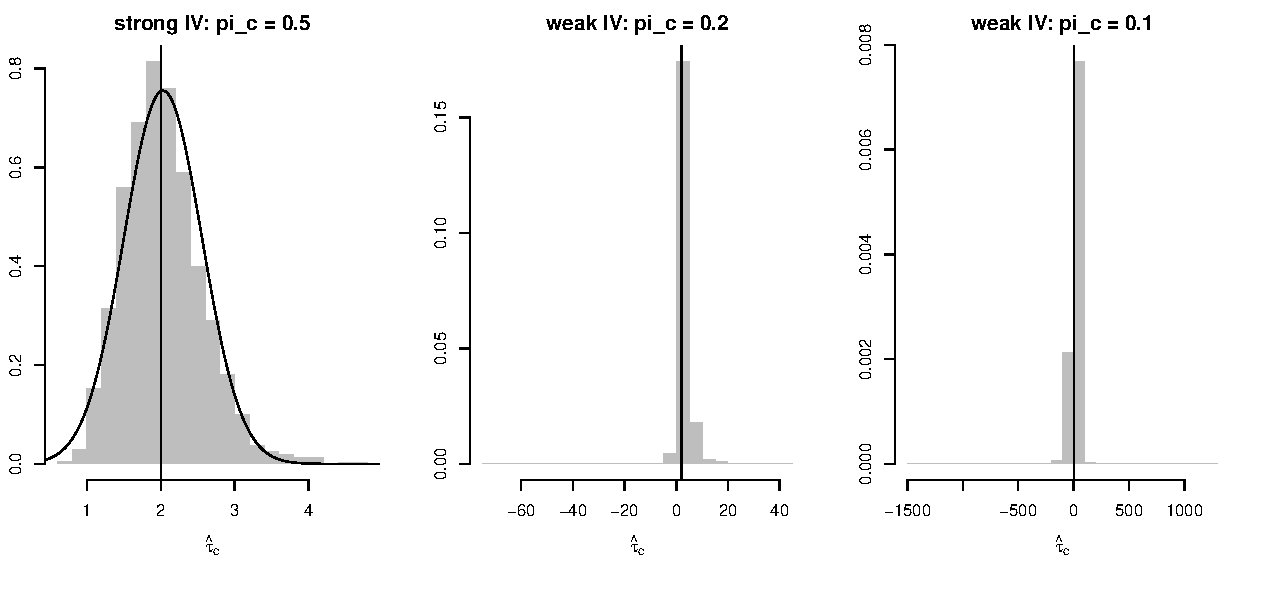
\includegraphics[width=\textwidth]{figures/wald_simulation.pdf}
                \caption{不进行协变量调整}
                \label{fig::no-x-iv}
        \end{subfigure}%
        
        
        
        
        
        
\begin{subfigure}[b]{\textwidth}
                \centering
                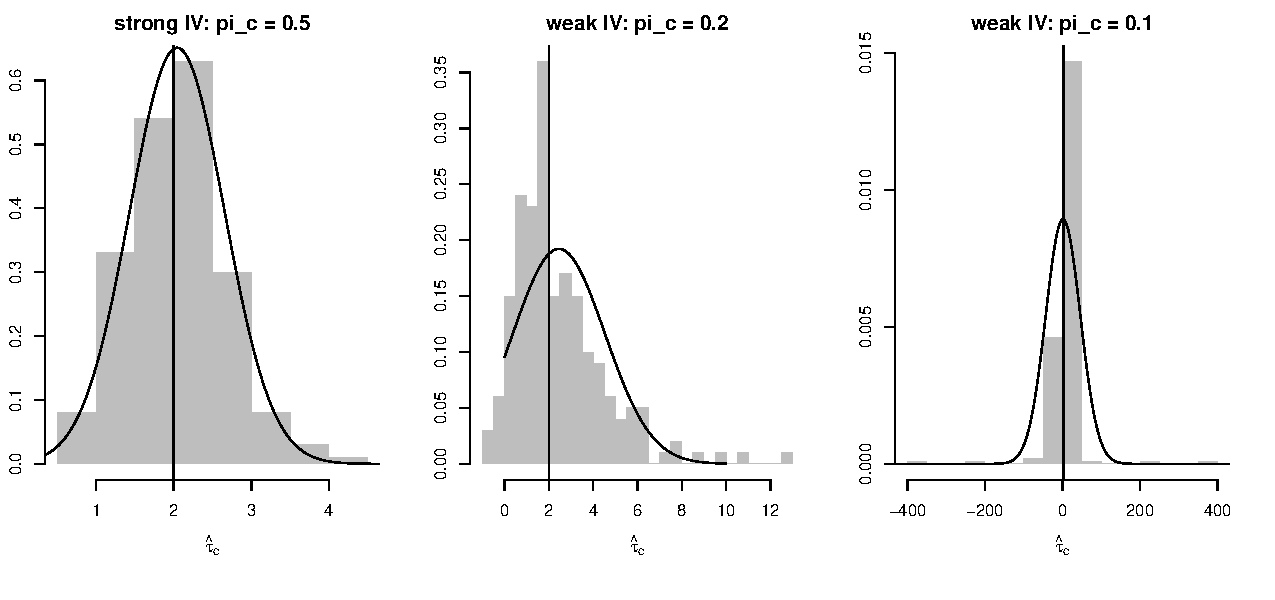
\includegraphics[width=\textwidth]{figures/waldX_simulation.pdf}
                \caption{进行协变量调整}
                \label{fig::x-iv}
        \end{subfigure}%        
\caption{强、弱工具变量的模拟}\label{fg::strong-weak-ivs}
\end{figure}


\subsection{鲁棒的置信区间构造}

如何处理弱工具变量？从检验角度看，解决办法很简单。由于$\tau_\cp = \tau_Y / \tau_D$，只要$\tau_D > 0$，下列两个零假设就等价：
$$
H_0: \tau_\cp  = 0 \Longleftrightarrow H_0': \tau_Y = 0
$$
因此，只需检验$H_0'$，即$Z$对$Y$的平均因果效应为零。这呼应了第\ref{sec::estimation-IV}节关于 ITT 分析与工具变量分析关系的讨论。 


从估计角度看，虽然点估计的有限样本性质较差，仍可以着重构造置信区间。由于$\tau_\cp = \tau_Y / \tau_D$，这个问题类似于经典的 Fieller--Creasy 问题。下面介绍受\citet{fieller1954some}启发的$\tau_\cp$置信区间构造方法，见第\ref{sec::fc-problem}节。利用置信区间与假设检验的对偶性（见第\ref{section::duality-ci-testing}节），可反演一系列零假设
$$
H_0(b): \tau_\cp = b . 
$$
来构造$\tau_\cp$的置信集合。在真实值$\tau_\cp = b$下，
$$
 \tau_Y  - b  \tau_D  = 0.
$$
所以零假设$H_0(b)$等价于结果$A_i( b) = Y_i - b  D_i $的平均因果效应为零：
$$
H_0(b): \tau_{A(b)} = 0 .
$$


令$ \hat{\tau}_A(b)$为$\tau_{A(b)} $的一般点估计量，$\hat{V}_A( b )$为对应方差估计量。其具体形式取决于研究设定。在不含协变量的完全随机实验中，$ \hat{\tau}_A(b)$是结果$A_i( b)$的均值差，$\hat{V}_A( b )$为 Neyman 型方差估计量。在含协变量的完全随机实验中，$ \hat{\tau}_A(b)$是\citet{lin2013}对结果$A_i( b)$提出的估计量，$\hat{V}_A( b )$是将$Y_i - b D_i$对$(Z_i, X_i, Z_i X_i)$作 OLS 回归得到的 EHW 方差估计，并加上第\ref{sec::cre-superpop}节讨论的修正项。\footnote{若采用有限总体视角，则不需要这个修正。}在无混杂观察性研究中，可以采用本书第\ref{part::observational-studies}部分的多种已有方法，估计$A_i( b)$上的平均因果效应及其方差。  


根据$ \hat{\tau}_A(b)$与$\hat{V}_A( b )$，可对$H_0(b)$构造 Wald 型检验。反演检验，就得到$\tau_\cp$的置信集合：
$$
\left\{  b:    \frac{   \hat{\tau}_A^2(b)  }{  \hat{V}_A(b)  } \leq z_{1-\alpha/2}^2 \right\}
$$
其中$z_{1-\alpha/2}$为标准正态分布的$1-\alpha/2$分位数。这与计量经济学中的 Anderson--Rubin 型置信区间\citep{anderson1950asymptotic}相近。考虑到它与\citet{fieller1954some}的联系，下面称其为 Fieller--Anderson--Rubin（FAR）置信区间。工具变量较强时，这些针对弱工具变量的区间退化为通常的渐近置信区间；工具变量较弱时，它们还能提供额外保证。我建议在实践中使用这些区间。 


\begin{example}\label{eg::FAR-CI-noX}
为直观理解 FAR 置信区间，考虑不含协变量的完全随机实验。区间中的二次不等式简化为
\begin{eqnarray*}
&& (\hat{\tau}_Y  - b   \hat{\tau}_D)^2 \\ 
& \leq & z_{1-\alpha/2}
\left[      n_1^{-1} \{  \hat{S}_Y^2(1)  + b^2\hat{S}_D^2(1) - 2 b \hat{S}_{YD}(1)  \}  \right. \\
&& \left. 
 + n_0^{-1} \{  \hat{S}_Y^2(0)  + b^2\hat{S}_D^2(0) - 2 b \hat{S}_{YD}(0)  \}    \right] ,
\end{eqnarray*}
其中$\{ \hat{S}_Y^2(1) ,  \hat{S}_D^2(1) , \hat{S}_{YD}(1)  \}$与$ \{ \hat{S}_Y^2(0), \hat{S}_D^2(0),\hat{S}_{YD}(0) \} $分别是处理组和对照组中$Y$、$D$的样本方差及协方差。置信集合可能是一个闭区间、两个不相连的区间、空集或整条实数轴。详细讨论留作习题\ref{para::FAR-CI-cases}。 
\end{example}
 



\subsection{实现与模拟}\label{sec::FARci-simulation}


下面的函数计算随$b$变化的一系列$p$值。\ri{FARci}不使用协变量，\ri{FARciX}使用协变量，后者依赖第\ref{sec::simulation-CRE-superp}节定义的\ri{linestimator}函数。 

\begin{lstlisting}
FARci = function(Z, D, Y, Lower, Upper, grid)
{
  CIrange = seq(Lower, Upper, grid)
  Pvalue  = sapply(CIrange, function(t){
    Y_t       = Y - t*D
    Tauadj    = mean(Y_t[Z==1]) - mean(Y_t[Z==0])
    VarAdj    = var(Y_t[Z==1])/sum(Z) + 
      var(Y_t[Z==0])/sum(1 - Z)
    Tstat     = Tauadj/sqrt(VarAdj)
    (1 - pnorm(abs(Tstat)))*2
  })
  
  return(list(CIrange = CIrange, Pvalue  = Pvalue))
}

FARciX = function(Z, D, Y, X, Lower, Upper, grid)
{
  CIrange = seq(Lower, Upper, grid)
  X       = scale(X)
  Pvalue  = sapply(CIrange, function(t){
    Y_t       = Y - t*D
    linest    = linestimator(Z, Y_t, X)
    Tstat     = linest[1]/linest[3]
    (1 - pnorm(abs(Tstat)))*2
  })
  
  return(list(CIrange = CIrange, Pvalue  = Pvalue))
}
\end{lstlisting}


图\ref{fg::FAR-ci-simulation}展示了不同$\pi_\cp$下模拟数据的$p$值随$b$变化的曲线。图\ref{fig::FARci-realization1}和\ref{fig::FARci-realization2}是同一数据生成过程的两次实现，细节见\ri{R}代码。图\ref{fig::FARci-realization1}中，FAR 置信集合都是闭区间；图\ref{fig::FARci-realization2}中，$\pi_\cp = 0.2$和$\pi_\cp = 0.1$时的置信集合则不是闭区间。$\pi_\cp = 0.5$时，置信集合的形状在两次实现中保持稳定。 



\begin{figure}
\centering 
\begin{subfigure}[b]{0.45\textwidth}
                \centering
                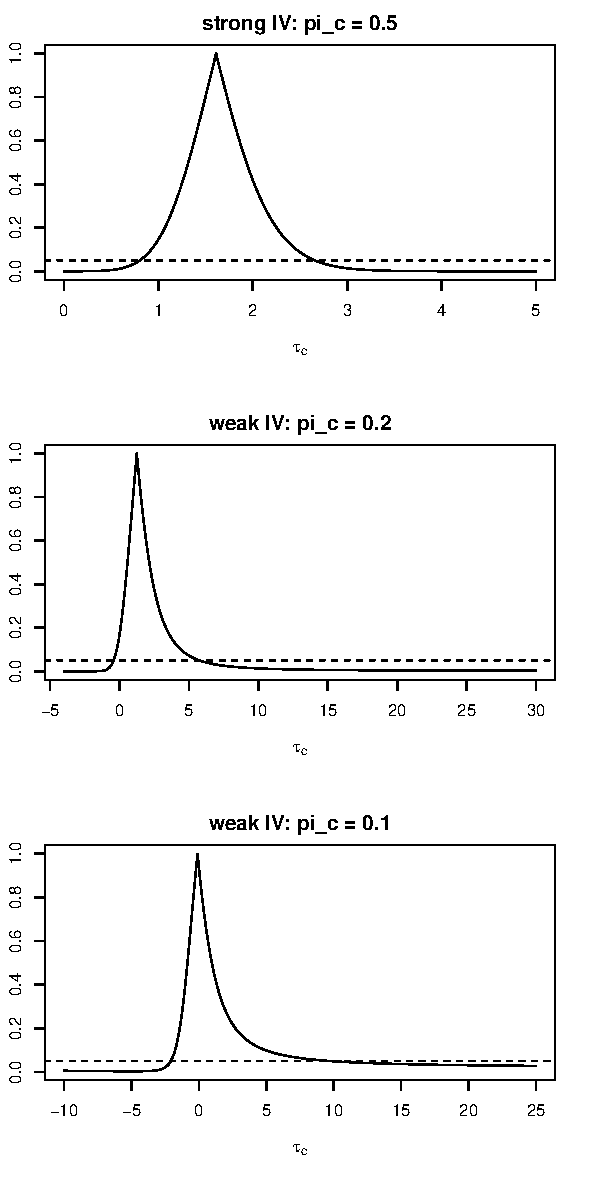
\includegraphics[width=\textwidth]{figures/FARci_simulation1.pdf}
                \caption{第 1 次实现}
                \label{fig::FARci-realization1}
        \end{subfigure}%
\begin{subfigure}[b]{0.45\textwidth}
                \centering
                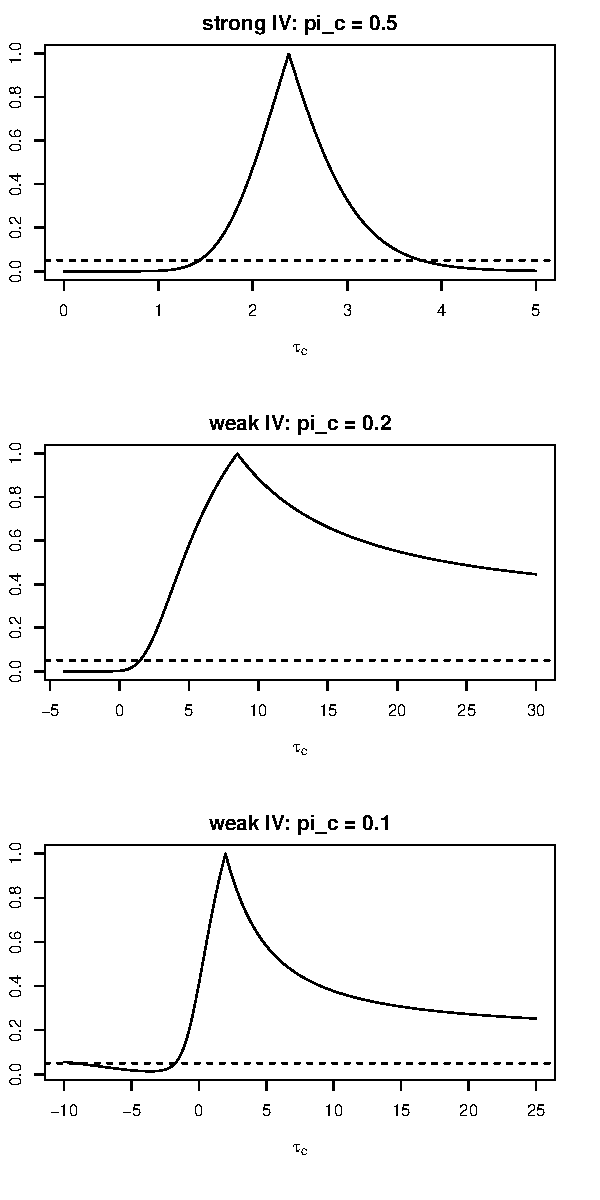
\includegraphics[width=\textwidth]{figures/FARci_simulation2.pdf}
                \caption{第 2 次实现}
                \label{fig::FARci-realization2}
        \end{subfigure}%        
\caption{不同$\pi_\cp$下模拟数据的 FAR 置信区间：两次实现}\label{fg::FAR-ci-simulation}
\end{figure}







\section{实例应用}
\label{sec::cace-application}


\ri{mediation}包中的\ri{jobs}数据集来自求职干预研究 JOBS II，这是一项研究职业培训干预对失业者成效的随机实地实验。\ri{treat}表示参与者是否被随机选入 JOBS II 培训项目，\ri{comply}表示是否实际参加。一个关注的结果是\ri{job_seek}，用于衡量求职自我效能感，取值为 1 至 5。协变量包括\ri{sex}、\ri{age}、\ri{marital}、\ri{nonwhite}、\ri{educ}和\ri{income}。 

 \begin{lstlisting}
> jobsdata = read.csv("jobsdata.csv")
> Z = jobsdata$treat
> D = jobsdata$comply
> Y = jobsdata$job_seek
> getX     = lm(treat ~ sex + age + marital 
+               + nonwhite + educ + income,
+               data = jobsdata)
> X = model.matrix(getX)[, -1]
\end{lstlisting}


可用$\hat{\tau}_\cp$估计$\tau_\cp$，并分别根据$\hat{V}_{\hat{A}}$和自助法计算标准误。还可进行协变量调整，得到$\hat{\tau}_{\cp,\textsc{L}}$，并用自助法估计标准误。结果如下，各方法的点估计与标准误都较稳定。 
 \begin{lstlisting}
> ## without covariates
> res = rbind(IV_Wald_delta(Z, D, Y),
+             IV_Wald_bootstrap(Z, D, Y, n.boot = 10^3))
> ## with covariates 
> res = rbind(res, 
+             IV_Lin_bootstrap(Z, D, Y, X, n.boot = 10^3)) 
> res = cbind(res, res[, 1] - 1.96*res[, 2],
+             res[, 1] + 1.96*res[, 2])
> row.names(res) = c("delta", "bootstrap", "with covariates")
> colnames(res)  = c("est", "se", "lower CI", "upper CI")
> round(res, 3)
                  est    se lower CI upper CI
delta           0.109 0.081   -0.050    0.268
bootstrap       0.109 0.083   -0.054    0.271
with covariates 0.118 0.082   -0.042    0.278
\end{lstlisting}



也可通过反演检验构造 FAR 置信集合，结果与上述置信区间类似。 
 \begin{lstlisting}
                   lower CI upper CI
without covariates   -0.050    0.267
with covariates      -0.047    0.282
\end{lstlisting}

图\ref{fig::FAR-p-value}给出了一系列检验的$p$值。 

\begin{figure}[ht]
\centering
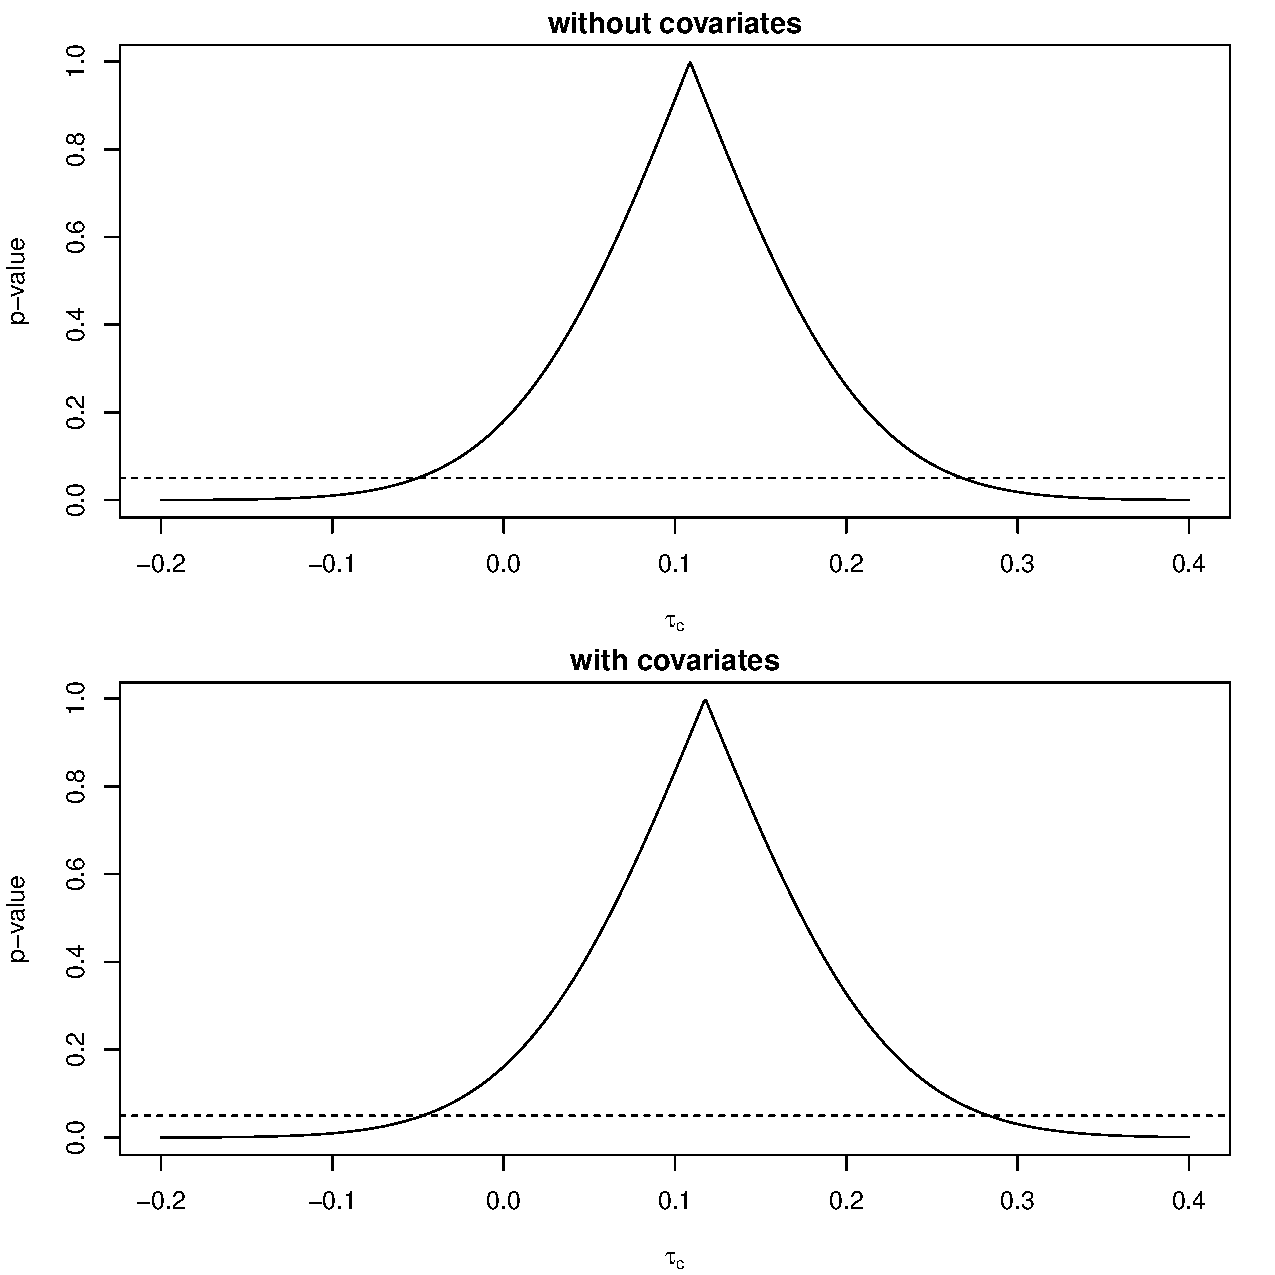
\includegraphics[width = \textwidth]{figures/farci_jobs.pdf}
\caption{通过反演检验构造的$\tau_\cp$置信区间：上图未调整协变量，下图调整了协变量}\label{fig::FAR-p-value}
\end{figure}




\section{CACE 的解释}\label{eq::interpret-iv-double}

潜在结果$\{ D(1), D(0), Y(1), Y(0)  \}$是针对处理分配$Z$这一假想干预定义的，因此$\tau_\cp$是依从者中处理分配对结果的平均因果效应。幸运的是，依从者满足$D=Z$，所以也可以把$\tau_\cp$解释为依从者中实际接受的处理对结果的平均因果效应。这部分回答了科学研究的问题。 

 

一些论文使用不同记号。例如，\citet{angrist1996identification}在一个二乘二析因实验中，用$Y_i(z,d)$表示单位$i$在处理分配为$z$、实际接受处理为$d$时的潜在结果。\footnote{“析因实验”这一名称来自实验设计文献\citep{dasgupta2014causal}，指实验者向每个单位随机分配多个因子，因而处理有多个水平。}\citet[][Section 3.1]{angrist2022empirical}回顾了采用这一记号的学术渊源。在此记号下，排除限制可表述如下。



\begin{assumption}[排除限制]
\label{assume::ER-double-index}
对所有$i$，有$Y_i(z,d) = Y_i(d)$，即潜在结果仅为$d$的函数。
\end{assumption}


由下面的因果图可见，假设\ref{assume::ER-double-index}排除了$Z$到$Y$的直接箭头。在这种情况下，$Z$是$D$的工具变量。 
\begin{center}
$
\xymatrix{
 && & U  \ar[dl] \ar[dr] &\\
Z \ar[rr] &&D \ar[rr]&&Y
}
$
\end{center}
在假设\ref{assume::ER-double-index}下，扩展记号$Y_i(z,d)$简化为$Y_i(d)$，这也解释了“排除限制”的名称。因此，对$d=0,1$有$Y_i(1,d) = Y_i(0,d)$；结合假设\ref{assume::Mono}，可得
\begin{eqnarray*}
Y_i(z=1) - Y_i(z=0) &=& Y_i(1, D_i(1)) - Y_i(0, D_i(0)) \\
&=& \left \{ \begin{array} {ll}
0 , & \text{if} \hspace{2mm}  U_i = \at, \\
0 , & \text{if}  \hspace{2mm}  U_i = \nt,\\
Y_i(d=1) - Y_i(d=0) ,& \text{if} \hspace{2mm} U_i = \cp.
\end{array}
\right.  
\end{eqnarray*}
这里特意区分潜在结果是针对$z$、$d$还是两者定义的，以免混淆。此前对$\tau_Y$的分解仍成立，从而得到\citet{imbens1994identification}和\citet{angrist1996identification}的以下结论。

回顾$D$上的平均因果效应$\tau_D = E\{D(1)  - D(0) \},$，再将$Y$上的平均因果效应定义为$\tau_Y = E\{ Y(D(1)) - Y(D(0))  \}$，将依从者平均因果效应定义为
$$
\tau_\cp =  E\{  Y(d=1) - Y(d=0) \mid U = \cp \}.
$$

\begin{theorem}\label{thm::iv-double-index}
在假设\ref{assume::Mono}至\ref{assume::ER-double-index}下，有
$$
Y(D(1)) - Y(D(0)) = \{  D(1)  - D(0) \} \times \{ Y(d=1) - Y(d=0) \}
$$
以及
$
\tau_\cp   =   \tau_Y /  \tau_D  .
$
\end{theorem}

除记号的相应调整外，证明与定理\ref{thm::CACE-identification}几乎相同，留作习题\ref{para::iv-alternative-form-theorem}。使用记号$Y_i(d)$，更便于将$\tau_\cp$解释为依从者中实际接受处理对结果的平均因果效应。 



 




 
\section{作业习题}



 
\paragraph{Wald 估计量的方差问题}\label{problem::infinite-var-iv}

证明 $\var(\hat{\tau}_\cp) = \infty$。 



\paragraph{Wald 估计量渐近方差及其估计}\label{problem::var-iv-estimate}


考虑$n\rightarrow \infty$的大样本情形。先证明$\sqrt{n}(\hat{\tau}_\cp - \tau_\cp) \rightarrow \textsc{N}(0, V)$依分布收敛，并求出$V$；再证明$\hat{V}_{\hat{A}} /V \rightarrow 1$依概率收敛。 

 
 
 
\paragraph{\citet{imbens1994identification}与\citet{angrist1996identification}的主要定理的证明} 
 \label{para::iv-alternative-form-theorem}
 
 证明定理 \ref{thm::iv-double-index}。 
 


\paragraph{FAR 置信区间的类型判别}\label{para::FAR-CI-cases}

例\ref{eg::FAR-CI-noX}中的置信集合可以是一个闭区间、两个不相连的区间、空集或整条实数轴。分别求出每种情形的确切条件。
 
 
 \paragraph{含协变量 FAR 模拟}\label{para::FAR-CI-simulation-X}

图\ref{fg::FAR-ci-simulation}给出了不使用协变量的 FAR 置信集合。对完全随机实验中调整协变量后的 FAR 置信集合进行类似模拟。 
 
 
\paragraph{序数型处理情形分析}\label{para::iv-ordinal-treatment}

\citet{angrist1995two}讨论了一种更一般的设定：工具变量$Z$为二元变量，实际接受的处理$D \in \{0,1,\ldots, J\}$为有序变量，结果为$Y$。相对于二元工具变量，实际接受处理有潜在取值$D(1)$与$D(0)$；相对于工具变量和实际接受处理的联合干预，结果有潜在取值$Y(z,d)$。将第\ref{eq::interpret-iv-double}节及相应工具变量假设推广如下。

\begin{assumption}\label{assumption::iv-ordinal-treatment}
有以下假设：(1) 随机化，$Z\ind \{   D(z),  Y(z,d)  : z=0,1; d = 0,1,\ldots, J \}$；(2) 单调性，$D(1) \geq D(0)$；(3) 排除限制，对所有$z=0,1$和$ d = 0,1,\ldots, J $均有$Y(z,d) = Y(d)$。 
\end{assumption}

他们证明了下面的定理 \ref{thm::iv-ordinal-treatment}。

\begin{theorem}\label{thm::iv-ordinal-treatment}
在假设\ref{assumption::iv-ordinal-treatment}下，
$$
\frac{  E(Y\mid Z=1) - E(Y\mid Z=0) }{ E(D\mid Z=1) - E(D\mid Z=0)  }
= \sum_{j=1}^J  w_j E\{  Y(j) - Y(j-1)  \mid D(1) \geq j > D(0) \}
$$
其中
$$
w_j = \frac{   \pr\{  D(1) \geq j > D(0)   \}   }{   \sum_{j'=1}^J  \pr\{  D(1) \geq j' > D(0)   \}   }.
$$
\end{theorem}



证明定理 \ref{thm::iv-ordinal-treatment}。

注：$J=1$时，定理\ref{thm::iv-ordinal-treatment}退化为定理\ref{thm::iv-double-index}。对于一般的$J$，标准工具变量公式识别的是若干潜在亚组效应的加权平均。权重与由$  D(1) \geq j > D(0) $定义的潜在亚组的概率成正比，亚组效应$E\{  Y(j) - Y(j-1)  \mid D(1) \geq j > D(0) \}$比较实际接受处理的相邻水平。但这些潜在亚组相互重叠，因此这一加权平均未必容易解释。



证明可能较为繁琐。一个技巧是，将处理分配为$z$时实际接受的处理与结果写为
$$
D(z) = \sum_{j=0}^J j 1\{ D(z) = j\} ,\quad 
Y(D(z)) = \sum_{j=0}^J  Y(j)1\{ D(z) = j\} 
$$
从而得到
$$
D(1) - D(0) = \sum_{j=0}^J j [ 1\{ D(1) = j\} -1\{ D(0) = j\} ]
$$
以及
$$
 Y(D(1))  - Y(D(0))   = 
\sum_{j=0}^J Y(j)   [ 1\{ D(1) = j \}   - 1\{ D(0) = j \}  ].
$$
再对适当选定的序列$(f_j)$与$(g_j)$，应用下面的{\it Abel 引理}，也称{\it 分部求和公式}：
$$
\sum_{j=0}^J  f_j (g_{j+1} - g_j) 
= 
f_J g_{J+1} - f_0 g_0  - \sum_{j=1}^J g_j  (f_j - f_{j-1})
$$ 





 
 


\paragraph{数据分析：流感疫苗接种鼓励设计\citep{mcdonald1992effects}}\label{problem::flushot}
 

\ri{fludata.txt}数据集来自\citet{mcdonald1992effects}的一项随机鼓励设计，\citet{hirano2000assessing}也重新分析过这一数据集。其变量如下：

\begin{tabular}{ll}
\hline 
\texttt{assign} & 是否受到接种流感疫苗鼓励的二元指标\\
\texttt{receive} & 是否实际接种流感疫苗的二元指标 \\
\texttt{outcome} & 是否因流感相关原因住院的二元结果\\
\texttt{age} & 患者年龄\\
\texttt{sex} & 患者性别\\
\texttt{race} & 患者种族\\
\texttt{copd} &  慢性阻塞性肺病\\
\texttt{dm} & 糖尿病\\
\texttt{heartd} & 心脏病\\
\texttt{renal} & 肾病\\
\texttt{liverd} & 肝病\\
\hline 
\end{tabular}


分析随机干预实验数据。 
 


\paragraph{基于协变量的 IV 估计}\label{hw::iv-conditional-x}

在\ri{R}中实现第\ref{section::unconfounded-IV}节提到的估计量及其方差估计量。 

注：本题有助于完成习题\ref{hw::analyze-karolinska-iv}。 



\paragraph{Karolinska 数据再分析}\label{hw::analyze-karolinska-iv}

重新考虑习题\ref{hw::Karolinska-dr}。\citet{rubin2008objective}用 Karolinska 数据说明工具变量方法。在\texttt{karolinska.txt}中，是否在高诊疗量医院确诊，可视为是否在高诊疗量医院接受治疗的工具变量。在给定其他观测协变量后，这一设定是合理的，详见\citet{rubin2008objective}的分析。 


基于观测数据验证工具变量法的有效性。 

 
 
 \paragraph{数据分析：职业培训项目}

文件\texttt{jobtraining.rtf}说明了数据文件\texttt{X.csv}与\texttt{Y.csv}的内容。 

\texttt{X.csv}包含处理前协变量。也可以将抽样权重变量\texttt{wgt}视为一个协变量；许多既有分析都采用了这种简化，尽管它在调查数据分析中始终存在争议。请分别进行调整与不调整协变量的分析。 

\texttt{Y.csv}包含抽样权重、处理分配、实际接受的处理以及许多处理后变量。因此，根据研究问题不同，可以选择多种结果。数据还存在若干复杂之处：一些结果缺失；失业者没有工资；结果还在多个时间点重复观测。分析时，请详细说明研究问题与估计量的选择。 

注：\citet{schochet2008does}分析了原始数据。\citet{frumento2012evaluating}根据后文第\ref{chapter::principal-stratification}章的框架，进行了更复杂的分析。 


 \paragraph{推荐阅读}

\citet{angrist1996identification}将计量经济学中的工具变量视角与基于潜在结果的统计因果推断联系起来，并通过一个应用说明了这一联系的价值。 

工具变量方法的其他早期文献还包括\citet{permutt1989simultaneous}、\citet{sommer1991estimating}、\citet{baker1994paired}和\citet{cuzick1997adjusting}。 


